% Created 2019-01-06 Sun 02:40
\documentclass[12pt,a4wide]{article}
\usepackage[utf8]{inputenc}
\usepackage[T1]{fontenc}
\usepackage{fixltx2e}
\usepackage{graphicx}
\usepackage{longtable}
\usepackage{float}
\usepackage{wrapfig}
\usepackage{rotating}
\usepackage[normalem]{ulem}
\usepackage{amsmath}
\usepackage{textcomp}
\usepackage{marvosym}
\usepackage{wasysym}
\usepackage{amssymb}
\usepackage{hyperref}
\tolerance=1000
\usepackage{french}
\setlength{\oddsidemargin}{0cm}
\setlength{\evensidemargin}{0cm}
\setlength{\textwidth}{500pt}
\author{Stephane Genaud}
\date{\today}
\title{aroma}
\hypersetup{
  pdfkeywords={},
  pdfsubject={},
  pdfcreator={Emacs 25.1.1 (Org mode 8.2.10)}}
\begin{document}

\maketitle
\begin{export}
\begin{titlepage}
\begin{center}
{\large Mémoire du Diplôme d'Université d'Aromathérapie \par}
\vspace{.7cm}
{\Large \emph{Les huiles essentielles pour la répulsion des tiques} \par}
\vspace{2cm}
{\large Sophie \textsc{Genaud} \par}
\vspace{2cm}
{\Large  \par}
\end{center}
\vfill
\begin{center}

{
\includegraphics[width=4cm]{img/logo-uB-filet.png} \par}
{\large Janvier 2018}
\end{center}
\end{titlepage}

\tableofcontents
\newpage
\end{export}






\section{Introduction}
\label{sec-1}

\paragraph{Le Contexte}
\label{sec-1-0-0-1}
Des scandales  sanitaires à répétition  et une remise  en question de  notre vie
actuel  ont été  à l'origine  d'un regain  d'intérêt pour  les médecines  et les
traitements naturels.Des étude scientifiques de  plus en plus nombreuses mettent
peu à peu à mal nos croyances relatives à notre santé et à la toute puissance de
la médecine  ``moderne'' avec  ses médicaments  synthétiques.  Dans  ce contexte
beaucoup sont  tentés de soigner leurs  maux quotidiens par la  phytothérapie ou
l'aromathérapie perçues comme plus naturelles.
\emph{Les huiles essentielles c'est sans danger puisque c'est naturel} !
Combien de fois avons nous entendu ce discours dans notre exercice officinal !
Leur usage est souvent banalisé par leur appellation ``produit naturel''.\\


Le danger  actuel réside en une  règlementation floue permettant de  se procurer
des huiles  essentielles en  Officine certes  mais aussi  en grande  surface, en
magasin ``bio'' ou encore sur internet. Il est de notre éthique de Pharmacien de
s'assurer que les  huiles essentielles que nous conseillons  seront employées de
la  façon  la  plus  sûre  et  la plus  efficace  possible.   C'est  dans  cette
perspective qualitative que  nous avons abordé ce DU d'Aromathérapie  qui nous a
permis  d'aller  beaucoup plus  loin  dans  nos connaissances,  nous  permettant
dorénavant :
\begin{itemize}
\item d'avoir une approche biochimique indispensable pour comprendre la relation
structure- activité d'une huile essentielle,
\item de conseiller en toute sécurité en se basant sur les familles biochimiques
permettant de bien comprendre les indications et les contre-indications,
\item d'avoir une  esprit critique par rapport  aux formules existantes tant  par le
choix des huiles que par leurs concentrations,
\item d'élaborer à partir de nos propres connaissances nos formules en fonction de
la symptomatologie précise de notre patient pour une réponse plus
personnalisée,
\item d'exercer donc en toute sécurité pour notre patient et pour notre
éthique propre, en prenant en compte les contraintes réglementaires et
juridiques actuels.\\
\end{itemize}


\paragraph{Sujet du mémoire}
\label{sec-1-0-0-2}
Dans ce  mémoire nous  avons choisi  de traiter un  problème auquel  nous sommes
confrontés chaque année, le retour des tiques  et avec elles la Maladie de Lyme.
Je  suis titulaire  d'une Officine  en  Alsace –à  Metzéral- dans  la Vallée  de
Munster et nous  observons de plus en plus  de cas au fil des  ans. Nous voulons
élaborer  un spray  répulsif pour  les  adultes, pour  les enfants  et pour  les
chiens. Nous  voulons également aller  plus loin et suite  à ce DU  nous voulons
proposer une solution à appliquer et une solution à prendre par voie orale après
la morsure.


Nous aborderons ce mémoire en trois chapitres.


Le premier portera sur un rapide rappel de la maladie, sur la pertinence de ce
choix par rapport à ma situation géographique et sur les mesures préventives
indispensables à mettre en place.

Le deuxième chapitre repertoriera les familles biochimiques anti-parasitaires, 
ayant des propriétés larvicides, ovicides et répulsives. Ce DU d'aromathérapie
m'a donné envie d'aller plus loin et de chercher des études scientifiques
prouvant l'efficacité des huiles essentielles dans ces indications.

Le troisième chapitre reprendra les résultats du précédent et permettra
d'établir les formules définitives que je compte mettre en pratique à l'Officine
au printemps.





\section{Qu'est-ce que la maladie de Lyme ?}
\label{sec-2}
 La maladie  de Lyme  ou \emph{borréliose  de Lyme}  est une
maladie infectieuse due  à une bactérie appelée  Borrelia burgdorferi, transmise
par l'intermédiaire d'une  piqûre de tique infectée. Après
 l'inoculation cutanée de la bactérie lors de  la piqûre de tique, la maladie de
 Lyme évolue en trois grandes  phases, séparées par des périodes asymptomatiques
.  Lorsqu'elle n'est pas traitée,  la maladie
 peut mettre plusieurs années à se développer. Les chercheurs parlent de maladie
 émergente, car les cas sont de plus en plus nombreux. (2 )

\section{Description de la maladie et symptomatologie}
\label{sec-3}
\subsection{La phase primaire de la maladie de Lyme}
\label{sec-3-1}

Elle est caractérisée par une lésion cutanée : l'érythème chronique migrant (ECM). Cette lésion survient ente 3 et 30 jours après la piqûre de tique. Il s'agit d'une papule érythémateuse (rouge) centrée par le point de piqûre, s'étendant progressivement de façon centrifuge. La lésion est ovale (pouvant mesurer jusqu'à 50 cm), la bordure est plus érythémateuse (rouge) que son centre qui retrouve progressivement un aspect cutané normal. Elle est habituellement non prurigineuse (absence de grattage) et siège préférentiellement aux membres inférieurs (parfois aux membres supérieurs, voire au visage chez l'enfant). En l'absence de traitement, l'ECM évolue pendant quelques semaines (extension progressive) et disparaît sans séquelle.


Durant cette première phase, vous pourrez constater des Maux de tête, Poussées de fièvre, Frissons, Douleurs articulaires et musculaires Fatigue.
Il est à noter que 20\% des personnes atteintes par cette maladie, l'ECM reste très discret, disparait au bout d'un mois et l'individu n'aura pas remarqué sa présence. La maladie de Lyme passera totalement inaperçue et aucun traitement n'aura été pris. Ces cas peuvent être graves, puisque la maladie pourra se compliquer durant la seconde phase.



\subsection{La phase secondaire de la maladie de Lyme}
\label{sec-3-2}

Elle survient plusieurs semaines ou mois après la disparition de l'ECM mais peut révéler la maladie (l'ECM étant passé inaperçu ou pouvant manquer dans près de la moitié des cas). Cette phase se caractérise par :
\begin{itemize}
\item Des manifestations cutanées : il s'agit de lésions semblables à celles observées lors de la phase primaire de la maladie ;
\item Des manifestations articulaires : douleurs articulaires fréquentes. Les arthrites (inflammation des articulations) sont moins fréquentes et touchent les grosses articulations (genou) ;
\item Des manifestations cardiaques : syncopes, palpitations, douleurs thoraciques et surtout troubles de la conduction auriculo-ventriculaire

\item Des manifestations neurologiques : la radiculite hyper-algique (inflammation très douloureuse des racines des nerfs innervant le territoire de la piqûre de tique). Le nerf facial est fréquemment touché. Une méningite peut également s'observer. 

Il devient primordial de traiter la maladie, sans quoi la troisième phase pourrait se développer, des années plus tard pour certains individus, dans des conditions pouvant être très graves.
\end{itemize}


\subsection{La phase tertiaire de la maladie de Lyme}
\label{sec-3-3}

Si la maladie de Lyme n'a pas été traitée au cours des deux premières phases, la
troisième pourrait  se révéler fatale  à l'individu infecté. Tous  les symptômes
précédemment  cités s'aggraveront  doucement, devenant  chroniques, au  cours de
cette dernière  phase qui  peut se manifester  des mois ou  des années  après le
début de l'infection par :

\begin{itemize}
\item Des  atteintes cutanées  :  la maladie  de  Pick Herxheimer  (inflammation
cutanée évoluant  vers une  atrophie de la  peau), le  lymphocytome cutané
bénin (nodules violacés,  arrondi, à contours nets,  fermes, localisés sur
le  front, le  lobe de  l'oreille et  régressant spontanément  en quelques
mois) ;

\item Des atteintes articulaires : identiques à celles observées dans la phase secondaire ;
\item Des atteintes neurologiques : touchant la moelle épinière ou le cerveau (manifestations neuro-psychiatriques diverses).
\end{itemize}

Tous les organes pourront être infectés et s'étendront au niveau des nerfs, des yeux, des articulations jusqu'à contaminer le cœur et la rate. De plus, des atrophies de parcelles de peau pourra être constaté. Celle-ci deviendra très fines, voire transparentes et donnera un effet papier froissé tirant sur les rouges violets. Les conséquences cardiaques pourront aussi être grave en fonction des infections.
A noter que l'évolution vers cette troisième phase reste extrêmement rare, même dans le cas où l'individu n'aura pris aucun traitement.


\subsection{Diagnostic de la maladie de Lyme}
\label{sec-3-4}

Comme nous l'avons vu ci-dessus, il est très difficile de diagnostiquer la maladie de Lyme. Les symptômes peuvent être très nombreux mais aussi indolores voire presque «invisibles». De plus, il est très facile de confondre les symptômes décrits avec d'autres maladies. Lorsque l'on constate ces symptômes, il est conseillé d'aller chez le médecin rapidement et d'indiquer si vous avez été mordu par une tique. Lorsque l'individu ne sait pas s'il a été piqué par une tique, il pourra indiquer au médecin s'il a été dans des endroits susceptibles de contenir des tiques ; lors de balades en forêt par exemple. 
 Il est à noter que les prises de sang ne permettent pas toujours de valider la présence de l'infection, surtout si le patient est toujours dans le premier stade de la maladie. Le médecin pourra aussi effectuer un électrocardiogramme afin de rechercher d'éventuels troubles auriculo-ventriculaire. Dans ces cas, une hospitalisation du patient devra être effectuée.
Dans les cas avancés de la maladie de Lyme, soit à partir de la seconde phase, des examens neurologiques seront nécessaires. Ils permettront de mettre en évidence une diminution des sensations, des forces musculaires ainsi que d'éventuels inflammation des nerfs. En cas de radiculite (phase secondaire), cet examen peut être normal ou mettre en évidence une diminution de la sensibilité, une diminution de la force musculaire ou une abolition des réflexes dans le territoire innervé par le nerf touché par l'inflammation.
Le diagnostic de la maladie de Lyme repose essentiellement sur les signes cliniques observés.
La numération formule sanguine est normale le plus souvent.
Diverses techniques de laboratoire peuvent mettre en évidence dans le sang des anticorps témoins d'une réponse de l'organisme à l'infection bactérienne. Les tests immunologiques les plus récents sont à privilégier.

En cas d'atteinte neurologique, la présence d'anticorps dans le liquide céphalo-rachidien est un argument en faveur de la maladie de Lyme.


\subsection{Traitement de la maladie de Lyme}
\label{sec-3-5}

La prise d'antibiotiques est obligatoire pour soigner l'infection causée par les tiques. le traitement et les dosages pourront être modifiés en fonction du temps passé depuis l'infection, et donc de la phase de la maladie. La prise d'antibiotique devra se faire sur une durée minimale de deux semaines pouvant aller jusqu'à trois suivant les zones impactées par l'infection.
Dans les cas les plus avancées de la maladie, des antibiotiques pourront être
administrés par voie intraveineuse sur des durées pouvant être beaucoup plus
longues. Dans les cas d'hospitalisation, un corticoïde est souvent donné. 

C'est en délivrant une ordonnance d'antibiotiques souvent sur 21 jours que nous
savons que c'est un traitement contre la maladie de Lyme. Au fil des années nous
constatons au sein de l'officine de plus en plus de traitements. Nous avons même
eu un traitement l'an dernier au mois de décembre \ldots{} l'EMC était bien présent
et la personne ne se souvenait pas d'avoir enlevé une tique.






\subsection{Pertinence du sujet par rapport à ma région géographique (3) (4)}
\label{sec-3-6}


\subsubsection{Prévalence au niveau national}
\label{sec-3-6-1}

Le nombre des victimes de la Borrélia burgdorferi dans l'hexagone est maintenant estimé à 27 000 cas par an (\url{http://www.sante.gouv.fr/maladie-de-lyme.html}). Selon les données du Réseau Sentinelles, la prévalence moyenne est estimée à 43 cas pour 100 000 habitants depuis 2009. Entre 1999 et 2000, elle était à 16.5 cas pour 100 000 personnes et  entre 1988 et 1989, elle était à 9.4 cas pour 100 000 individus (\url{http://www.invs.sante.fr/Dossiers-thematiques/Maladies-infectieuses/Maladies-a-transmission-vectorielle/Borreliose-de-lyme/Donnees-epidemiologiques}). En se basant sur ces chiffres, il est facile de constater que  cette infection n'a cessé de gagner du terrain au niveau national.

\subsubsection{Incidence au niveau régional}
\label{sec-3-6-2}



Les études effectuées par les institutions impliquées dans la surveillance de la
maladie  de Lyme  ,  telle que  le  Réseau Sentinelles,  le  Centre National  de
Référence  des Borrélia  (CNR), l'InVS,  la Mutualité  Sociale Agricole  (MSA)…,
entre 1986 et 2012 ont permis  d'établir des taux d'incidence au niveau national
et régional.

\begin{figure}[htb]
\centering
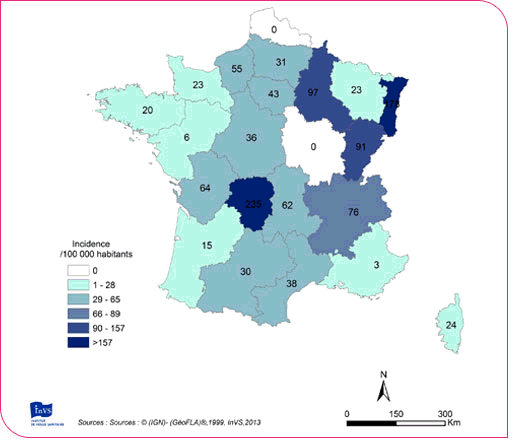
\includegraphics[width=.6\linewidth]{./img/carte_lyme.png}
\caption{Carte de France}
\end{figure}




On peut voir sur cette carte que l'incidence pour l'Alsace est dans cette étude de 157 cas pour 100 000 habitants, une incidence bien supérieure au taux moyen national.



D'autre part,  une étude de l'Agence  régionale de santé (ARS),  menée par Santé
publique  France et  grâce à  la participation  de 388  médecins, basée  sur des
critères européens, a permis d'affiner pour  la première fois les données. Mais
pas de miracle, la région Grand Est  constitue l'une des zones au plus fort taux
d'incidence de  borréliose de Lyme en  France.  2.200 cas de  borréliose de Lyme
par  an Tout  particulièrement concernés,  les deux  départements d'Alsace  dont
notamment les  secteurs situés à  proximité des massifs vosgiens.  Selon l'étude
baptisée Alsa  (ce) tique  et menée en 2014  et 2015, il y  aurait 2.200  cas de
borréliose de  Lyme en Alsace par  an soit un  taux d'incidence de 117  cas pour
100.000 habitants, une incidence deux fois supérieure au taux moyen national… La
majorité des personnes atteintes  dans le Grand Est sont des  hommes et 90 \% des
cas sont âgés de  16 ans ou plus, avec une moyenne de  55 ans. Chez les enfants,
les  5  à  9  ans  sont  les  plus touchés.  Si  les  lieux  à  risques  restent
principalement les  forêts (74 \%) les jardins  publics ou privés ne  sont pas en
reste (47 \%), tout comme les prairies (33 \%).


\subsection{Prévention de la maladie de Lyme}
\label{sec-3-7}

La maladie de Lyme est transmise à travers la piqûre, ou plus précisément la morsure, de tiques. Elle est transmissible chez l'Homme mais aussi chez de nombreux animaux. 
La prévention reste la première arme pour lutter contre cette maladie.
Des moyens simples existent :
    • porter des vêtements couvrants et clairs (afin de repérer rapidement les tiques), serrés au cou, aux poignets et aux chevilles (rentrer le bas du pantalon dans les chaussettes ou mettre des guêtres), des chaussures fermées et des gants clairs en cas de travail manuel ; 
    • vaporiser ses vêtements et ses chaussures de produits anti-tiques (en respectant les contre-indications pour les enfants et les femmes enceintes) ; 
    • utiliser un produit anti-tiques pour vos chiens et chats ; 
    • emprunter si possible les sentiers et marcher au milieu des chemins ; 
    • éviter les contacts avec les herbes, les broussailles et les branches basses ; 
    • inspecter le corps après une activité de travail ou de loisir en pleine nature (y compris le pli des genoux, les aisselles, les organes génitaux et le cuir chevelu) car la piqûre est indolore. Retirer rapidement la tique avec un tire-tique acheté en pharmacie, désinfecter et surveiller la zone de piqûre pendant plusieurs semaines ; 
    • consulter son médecin traitant en cas d'apparition de symptômes et en particulier d'une plaque rouge, centrée sur le point de piqûre et qui s'étend dans le mois qui suit la piqûre. 
Ce qu'il ne faut surtout pas faire (risque de régurgitation des agents infectieux) :
    • ne pas presser la tique entre ses doigts, afin de ne pas favoriser le passage de la salive de la tique qui contient les agents infectieux ; 
    • ne pas tirer sur la tique et ne pas utiliser de pince à épiler. Outre le risque précédent, la probabilité de ''laisser la tête'' dans la peau est forte. Cela provoque généralement une petite inflammation, une infection ou la formation d'un kyste ; 
    • ne pas utiliser d'alcool, d'éther, d'huile ou de vernis ; 
    • ne jamais tenter de brûler la tique avec un briquet. 


On l'aura bien compris la prévention est la première arme pour lutter contre la maladie.

\section{Choix des Huiles Essentielles}
\label{sec-4}

\subsection{Définition d'un produit insecticide/insectifuge}
\label{sec-4-1}
Une plante,  un produit ou  une substance est  insectifuge si elle  repousse les
insectes chez l'Homme  ou l'animal de compagnie ou d'élevage.  On parle aussi de
répulsif pour ces produits qui – par extension- désignent aussi des molécules ou
des produits commerciaux. ( wikipédia ) Un produit insecticide tue les insectes,
leurs larves  et/ou leurs  œufs tandis qu'un  produit insectifuge  les repousse.
Les insecticides font partie des pesticides, eux-mêmes inclus dans le groupe des
biocides, tous  règlementés en  Europe ( Fabienne  Millet revelessence.com  ) Le
terme générique  \emph{insecticide} est utilisé  pour citer les  produits pesticides,
les produits répulsifs agissant contre des arthopodes spécifiques : les insectes
( moustiques, mouches, punaises, poux, puces  , taons, fourmis ), les arachnides
( araignées, scorpions ), les acariens (tiques , aoûtats…).

\subsection{Mécanisme d'action}
\label{sec-4-2}
Ces produits agissent par contact ou par pénétration dans l'animal ( action systémique) et parfois par les deux mécanismes d'action.
Il est à noter que la tique n'a pas de perception visuelle contrairement à d'autres arthropodes. Elles sont équipées de récepteurs situés sur les pattes et non pas dans les antennes comme c'est souvent le cas. Sans vision elles s'orientent vers leurs hôtes , stimulées par leur odeur. La sensibilité à la température n'intervient pas car elles piquent aussi des animaux à sang froids ( serpents, lézards etc\ldots{})



Nous nous intéresserons donc aux huiles essentielles ayant une action insecticide  et insectifuge.
J'ai cherché des études prouvant l'efficacité des huiles essentielles dans ces indications pour les arthropodes d'une manière générale ( les tiques faisant partis de cette grande classe ). J'ai également trouvé quelques travaux portant directement sur les tiques.




\subsection{Les familles biochimiques}
\label{sec-4-3}

Toutes ces familles biochimiques sont bactéricides (anti-bactérien, anti-viral,
anti-fongique, anti-parasitaire), larvicides, acaricides et répulsives.

\subsubsection{Les monoterpenols}
\label{sec-4-3-1}

\begin{table}[htb]
\caption{Les monoterpenols}
\centering
\begin{tabular}{ll}
\textbf{Molécules} & \textbf{Huiles essentielles}\\
\textbf{chimiques} & \\
\hline
 & \\
Linalol & Bois de rose  (\emph{Aniba rosaeodora})\\
 & Thym ct linalol (\emph{Thymus vulgaris ct linalol})\\
 & Bois de Hô (\emph{Cinnamomum camphora ct linalol})\\
\hline
Citronellol & Géranium rosat (\emph{Pelargonium x asperum})\\
\hline
Géraniol & Palmarosa (\emph{Cymbopogon martinii})\\
 & Thym ct géraniol (\emph{Thymus vulgaris ct géraniol})\\
\hline
Thujanol & Thym ct thujanol \emph{(Thymus vulgaris ct thujanol)}\\
 & Marjolaine des jardins\\
 & ou à coquilles \emph{(Origanum majorana)}\\
\hline
Menthol & Menthe poivrée \emph{(Mentha x pipérita)}\\
 & Menthe des champs \emph{(Mentha arvensis)}\\
\hline
Terpinène 1 ol 4 & Tea Tree (\emph{Melaleuca alternifolia})\\
 & Marjolaine des jardins\\
 & ou à coquilles (\emph{Origanum majorana})\\
\hline
Alpha Terpinéol & Ravintsara (\emph{Cinnamomum camphora ct cinéole})\\
 & Niaouli (\emph{Melaleuca quinquenervia ct cinéole})\\
 & Eucalyptus radié (\emph{Eucalyptus radiata ssp radiata})\\
\hline
Bornéol & Thym à feuilles de sarriette (\emph{Thymus satureioides)}\\
 & Inule odorante (\emph{Inula graveloens})\\
\hline
 & \\
\end{tabular}
\end{table}


Ferreira  and  co, 2017  :Cette  étude  visait  à  comparer l'efficacité  du  N,
N-diéthyl-3-méthylbenzamide (DEET),  un répulsif standard,  au $\beta$-citronellol
dans un  dosage biologique par boîte  de Pétri. Un demi-cercle  de papier filtre
(31,8 cm2) a  été traité avec 87  ul de l'une des  quatre concentrations (0,200,
0,100,  0,050  et  0,025  mg  /  cm2)  de  $\beta$-citronellol,  DEET  ou  solvant
(éthanol). Un test  comparatif a été mis  au point en traitant un  côté avec des
concentrations  croissantes  de  $\beta$-citronellol, comme  mentionné  ci-dessus,
contre la concentration la plus élevée de DEET.  En outre, un test à blanc a été
effectué. Trois tiques  mâles et trois tiques femelles ont  été placés au milieu
d'un plateau et leur emplacement a été évalué 5, 10 et 30 minutes après le début
du  test.  En  conséquence, le  temps  n’a eu  aucun effet  significatif sur  la
réponse  de  répulsion  des  tiques  exposées  aux  deux  composés  et  à  leurs
concentrations. La réponse  répulsive augmente en fonction  de l'augmentation de
la concentration.  De plus,  les résultats  indiquent que  la tique  A. sculptum
était plus sensible  aux composés testés et que  le $\beta$-citronellol présentait
une efficacité supérieure à celle du DEET.

Jeyabalan  et al  (2003)  \footnote{DEFINITION NOT FOUND.}  ont étudié  l'effet  d'extraits  de feuilles  de
Pelargonium citrosa  sur Anopheles stephensi.  Les durées des  différents stades
larvaires et du développement global des larves sont augmentées. Ces différences
sont  notées   pour  toutes   les  concentrations  testées.   Des  malformations
apparaissent, et  la pupaison est incomplète  dans beaucoup de cas.   Toutes les
concentrations  en P.citrosa  ont  permis  la mise  en  évidence d'une  activité
repellent sur l'adulte de A. stephensi.  Aux concentrations les plus élevées, on
notait une  faiblesse des adultes et  des mouvements ralentis. Ces  mêmes effets
étaient  également retrouvés  sur  les larves.  Ces  résultats suggéraient  qu'à
partir  d'une   certaine  concentration,  les  repellents   avaient  des  effets
insecticides.  Enfin,  cette étude montrait  une diminution du nombre  de piqûre
sous l'effet de l'huile essentielle.


Iori et al  \cite{Iori2005} ont étudié l'effet acaricide  de l'huile essentielle
de  Melaleuca alternifolia  (Tea Tree)  sur  les nymphes  d'Ixodes ricinus.  Des
expériences ont  été réalisées à différentes  doses (4,6, 8  et 10 \$$\mu$\$l )  et pour
différents  temps  d'exposition   (30,  60,  90  et  120   min).  Des  résultats
intéressants ont  été obtenus après une  exposition de 90 minutes  avec un effet
renforcé lorsque la dose était augmentée à 10 \$$\mu$\$l.




\paragraph{Contre-indications}
\label{sec-4-3-1-1}
Déconseillé chez  la femme enceinte les  trois premiers mois de  la grossesse et
attention  à la  toxicité du  menthol chezle  jeune enfant.  Sinon, très  peu de
toxicité.



\subsubsection{Les phenols}
\label{sec-4-3-2}

\begin{table}[htb]
\caption{Les phenols}
\centering
\begin{tabular}{ll}
\textbf{Molécules chimiques} & \textbf{Huiles essentielles}\\
 & \\
\hline
Thymol & Thym ct thymol (\emph{Thymus vulgaris ct thymol})\\
\hline
Carvacrol & Origan compact (\emph{Origanum compaxtum})\\
 & Sariette des montagnes (\emph{satureja montana})\\
 & Thym ct carvacrol (\emph{Thymus vulgaris ct carvacrol})\\
 & Serpolet (\emph{thymus serpyllum})\\
\hline
Eugénol & Giroflier (clou) (\emph{Eugnenia caryphyllus})\\
 & Cannelle de Ceylan (\emph{Cinnamomum zeylannicum})\\
\hline
\end{tabular}
\end{table}


Tabari MA and co , 2017 ont étudié l'activité repellente d'une selection de monoterpènes (thymol, carvacrol et linalol ) contre Ixodes ricinus

Ils ont  évalué les effets ovicides,  larvicides et répulsifs contre  I. ricinus
des huiles essentielles du  thym, de la sarriette, de l'origan  de la lavande et
de  la  coriandre.   Des concentrations  de  0,25,  0,5,  1,  2 et  5\%  ont  été
pulvérisées sur les  masses d'oeufs, puis les taux d'éclosion  ont été notés. Le
carvacrol et  le thymol, à toutes  les concentrations testées, ont  entraîné une
diminution  significative de  l'éclosion, montrant  une efficacité  supérieure à
celle  de  la  perméthrine,  alors  que le  linalol  n'a  provoqué  aucun  effet
significatif. Chez les larves  traitées au carvacrol et au thymol  (1, 2 et 5\%),
les  taux de  mortalité ont  atteint 100\%  après 24  h, montrant  une efficacité
larvicide supérieure  à celle de  la perméthrine,  alors qu'aucun effet  n'a été
observé dans les groupes larvaires traités au linalol. Le carvacrol et le thymol
à  toutes  les  concentrations  testées   ont  montré  une  répulsion>  90\%  sur
I. ricinus.  Le linalol  n’était guère  efficace (répulsion  de 50,24\%)  qu’à la
concentration de  5\%. Globalement,  sur la  base de  ces résultats,  les phénols
carvacrol et thymol  peuvent être considérés comme des  ingrédients candidats au
développement de  nouvelles formulations acaricides permettant  de contrôler les
populations de  I. ricinus  et la  propagation des  maladies transmises  par les
tiques.


Viviane  Zeringóta, 2013  a étudié  l'activité  répulsive de  l'eugénol sur  des
larves  de  Rhipicephalus microplus  et  de  Dermacentor  nitens dans  un  essai
biologique. Les solutions ont été utilisées  à des concentrations de 10, 20, 30,
40 et 50 \$$\mu$\$l / ml.Pour les larves de D. nitens, la répulsion était supérieure
à 80\%  pendant une période  allant jusqu’à  5 h aux  concentrations de 40  et 50
\$$\mu$\$l /  ml; Pour les  larves de R.   microplus, les quatre  concentrations les
plus élevées ont produit des niveaux de  répulsion supérieures à 80\% pendant 9 h
au  plus. Par  conséquent,  l'eugénol  a une  activité  répulsive  sur le  stade
larvaire de ces  deux espèces de tiques,  les larves de R.  microplus étant plus
sensibles.



Pour Meng  and co,  2016 l'étude  portait sur  l'efficacité du  DEET et  de huit
huiles essentielles disponibles dans le commerce (origan, clou de girofle, thym,
vétiver, bois de  santal, cannelle, bois de cèdre et  menthe poivrée). Elles ont
été  évalués pour  leur pouvoir  de  répulsion contre  les nymphes  de la  tique
Amblyomma americanum. La répulsion de chaque  huile essentielle a été comparée à
celle  du N,  N-diéthyl-3-méthyl benzamide  (DEET).La concentration  efficace de
DEET qui repousse  50\% des tiques (CE50) a  été estimée à 0,02 mg  / cm2, tandis
que  la  CE50 des  huiles  essentielles  se situe  entre  0,113  et 0,297  mg  /
cm2. Selon  les estimations de la  CE 50, l'huile essentielle  d'origan était la
plus efficace parmi toutes les huiles  testées, suivie des huiles de girofle, de
thym, de vétiver, de bois de santal, de cannelle, de cèdre et de menthe poivrée.


Carol and co, 2017 : L'huile  essentielle d'origan, Origanum onites a été testée
dans  des essais  biologiques en  laboratoire visant  à déterminer  son activité
répulsive sur les tiques Amblyomma americanum et Aedes aegypti. Les composés les
plus abondants  de l'  HE d'Origanum  onites étaient  le carvacrol  (75,70\%), le
linalol (9,0\%), le p-cymène (4,33\%) et  le thymol (1,9\%). À une concentration de
0,413 mg d'huile / cm2 de  papier filtre, l'HE d'Origanum onites repoussait 100\%
des tiques  testées et  à 0,103  mg d'huile /  cm2 de  papier filtre,  66,7\% des
tiques étaient repoussées. À 0,075 mg d'huile  / cm2 de papier filtre, le thymol
a  repoussé  66,7\%  des  tiques,  contre  28,7\% pour  le  carvacrol  à  la  même
concentration.


\subsubsection{Les aldéhydes aromatiques}
\label{sec-4-3-3}

\begin{table}[htb]
\caption{Les aldéhydes aromatiques}
\centering
\begin{tabular}{ll}
\textbf{Molécules chimiques} & \textbf{Huiles essentielles}\\
 & \\
\hline
Cinnamaldéhyde & Cannelle de Ceylan (\emph{Cinnamomum zeylanicum})\\
 & Cannelle de Chine (\emph{Cinnamomum cassia})\\
 & Cannelle du Vietnam (\emph{Cinnamomum laureirii})\\
\hline
\end{tabular}
\end{table}




Paalson, 2008

L'effet répulsif des huiles essentielles des têtes de fleurs de la tanaisie de
la plante aromatique Tanacetum vulgare L. (Asteraceae), originaire de Suède, a
été testé sur des nymphes de la tique commune, Ixodes ricinus. Les principales
substances volatiles détectées dans les huiles de T. vulgare recueillies à
Uppsala étaient l’a-pinène (27\%), le $\beta$-pinène (11\%), le pinocamphone (11\%), le
1,3,3-triméthylcyclohex-1-énène-4-carboxaldéhyde. (11\%) et 1,8-cinéole
(10\%). Dans l'échantillon recueilli à Stockholm, les composants principaux
étaient la $\beta$-thujone (39\%) et le camphre (23\%), suivis de l'$\alpha$-thujone (11\%) et
du 1,8-cinéole (8\%). Lorsque les constituants des huiles, tels que
l'$\alpha$-terpinéol, le 4-terpinéol, l'$\alpha$ + $\beta$-thujone, le 1,8-cinéol, le verbénol et le
verbénone ont été testés séparément la répulsion a été de 64 \% à 72 \%.

\subsubsection{Etudes intéressantes}
\label{sec-4-3-4}


Katarína Štefanidesová and co, 2017 ont  étudié onze huiles essentielles sur les
tiques  Dermacentor reticulatus  ,  à savoir  le  basilic (Ocimum  basilicum),la
bergamote (Citrus bergamia),le bouton de  clou de girofle (Syzygium aromatic),la
citronnelle de  Java(Cymbopogon winterianus), le serpolet  (Thymus serpyllum),la
lavande (Lavandula  angustifolia),la marjolaine  (Origanum majorana),  la menthe
poivrée (Mentha piperita),  la menthe verte (Mentha spicata) et  le thym (Thymus
vulgaris). Ils ont  été soumis à des  tests de résistance à  la répulsion contre
les tiques adultes de D. reticulatus à des concentrations de 1 et 3\%. Les huiles
essentielles  de clou  de  girofle, de  serpolet  et de  thym  étaient les  plus
efficaces: 83, 82  et 68\% des tiques  ont été repoussées une fois  diluées à 3\%,
respectivement.  Le mélange  de serpolet  et  de citronnelle  contenant 1,5\%  de
chacun a  montré une  répulsion plus  élevée (91\%)  que les  huiles essentielles
individuelles à la concentration de 3\%.



Dans l'étude  \cite{El-Seedi2012} portant  sur l'efficacité de  répulsifs contre
les  tiques   d’origine  végétale,  les   auteurs  étudié  l’effet   des  huiles
essentielles  de quatre  plantes médicinales  et  culinaires de  la famille  des
Lamiaceae sur  les nymphes de la  tique Ixodes ricinus. Les  huiles essentielles
des  feuilles sèches  de  Rosmarinus officinalis  (Romarin),  de Mentha  spicata
(Menthe  verte),   d'Origanum  majorana  (Majoralaine)  et   d'Ocimum  basilicum
(Basilic) ont été isolée par distillation  à la vapeur avec une concentration en
huile de 15 microg / cm2. Elles ont  été testées contre les tiques dans un essai
biologique  en  laboratoire.  Les  huiles  de  R.  officinalis,  M.  spicata  et
O. majorana ont montré une forte répulsion contre les tiques 100, 93,2 et 84,3\%,
respectivement,   alors   que   O.   basilicum   n'a   montré   que   64,5\%   de
répulsion.  Lorsqu’ils   ont  été   testés  sur  le   terrain,  les   huiles  de
R. officinalis  et M. spicata ont  montré une répulsion  de 68,3 et 59,4\%  à une
concentration de  6,5 microg /  cm2 sur les tissus  d’essai. Les huiles  ont été
analysées par spectrométrie de masse par chromatographie en phase gazeuse et les
principaux composés  des huiles les  plus répulsives étaient le  1,8-cinéole, le
camphre, le linalol, le 4-terpinéol, le bornéol et le carvone.

\paragraph{Contre-indications}
\label{sec-4-3-4-1}
\begin{itemize}
\item La présence d'un noyau benzénique confère à ces molécules une dermo-causticité
au même titre que pour les phénols
\item Interdit chez la femme enceinte
\item Déconseillé chez l'enfant de moins de 7 ans
\end{itemize}

Une  dernière  étude slovaque  très  complète  nous  a interpellé.  Elle  étudie
l'efficacité de 11 huiles essentielles que nous avons déjà vues pour la plupart.


Ces onze  huiles essentielles,  à savoir  basilic (Ocimum  basilicum), bergamote
(Citrus bergamia),  bouton de clou  de girofle (Syzygium  aromatic), citronnelle
(Cymbopogon winterianus),  thym serpolet (Thymus serpyllum),  lavande (Lavandula
angustifolia),  la marjolaine  (Origanum  majorana), la  menthe poivrée  (Mentha
piperita), la  menthe verte (M. spicata)  et le thym vulgaire  (Thymus vulgaris)
ont  été soumis  à des  tests de  résistance à  la répulsion  contre les  tiques
adultes  de  D.  reticulatus  à  des  concentrations de  1  et  3\%.  Les  huiles
essentielles de clou de  girofle, de thym serpolet et de  thym rouge étaient les
plus efficaces: 83, 82  et 68\% des tiques ont été repoussées  une fois diluées à
3\%, respectivement. Le mélange de thym grimpant et de citronnelle contenant 1,5\%
de chacun a  montré une répulsion plus élevée (91\%)  que les huiles essentielles
individuelles à la concentration de 3\%.

\subsection{Le Basilic (Ocimum basilicum)}
\label{sec-4-4}

\subsubsection{Caractéristiques}
\label{sec-4-4-1}

\paragraph{Olfaction}
\label{sec-4-4-1-1}
Odeur fraîche, vive, anisée. Les premières notes rappellent l'estragon.
\paragraph{Propriétés}
\label{sec-4-4-1-2}

\begin{itemize}
\item Antispasmodique puissante
\item Calmante-relaxante
\item Antalgique
\item Antifongique
\item Tonique digestif
\item Anti-inflammatoire
\item Répulsive insectes
\end{itemize}

\paragraph{Indications}
\label{sec-4-4-1-3}
\begin{itemize}
\item Hoquet
\item Spasmes digestifs, coliques y compris néphrétiques
\item Ballonnements
\item Spasmophilie
\item Anxiété, insomnie, stress
\item Polyarthrite rhumatoïde
\item Eloigner les moustiques (en mélange avec d'autres huiles essentielles insectifuges)
\end{itemize}

\paragraph{Précautions d'emploi spécifiques}
\label{sec-4-4-1-4}
Huile  essentielle  réservée  à  l'adulte  et  sans  usage  répétitif.   L'huile
essentielle  de basilic  tropical présente  des précautions  spécifiques car  le
méthylchavicol  ou estragole  et  certains  de ses  dérivés  sont classés  comme
substance à fort potentiel toxique.  L'hépatocancérogénécité est démontrée chez  la souris et
la  toxicité hépatique  du  méthylchavicol est  mal déterminée  à  ce jour  chez
l'homme.  Une  recommandation européenne,  met en avant  la dose  journalière de
40mg par jour de méthylchavicol admissible par  voie orale pour un adulte ce qui
correspond à  une à  deux gouttes  toutes les 24  heures d'huile  essentielle de
basilic tropical.  Il convient d'éviter ou  de limiter la voie orale. Cet emploi
doit rester exceptionnel et restreint à une période très courte de 24 à 72H.  Il
est  préférable  de  privilégier  la  voie  cutanée  diluée  (huile  essentielle
irritante)   mais  toujours   sur   une   période  courte   (maximum   8  à   10
jours).  L'efficacité  par   cette  voie  est  très   importante.   Cette  huile
essentielle est  irritante pure sur la  peau. Il est indispensable  de la diluer
dans une huile végétale !  La  diffusion atmosphérique et les inhalations sèches
ne  posent pas  de problème  mais attention  à l'odeur  ! 

\subsubsection{Botanique}
\label{sec-4-4-2}

\paragraph{Description}
\label{sec-4-4-2-1}
Il existe de 50  à 150 espèces de basilic selon les sources.  Le basilic est une
plante annuelle touffue, de 20 à  60 centimètres de hauteur, pourvue de feuilles
ovales, de couleur vert  clair à vert foncé. Un sol riche  et bien drainé exposé
au soleil (plusieurs heures par jour) lui convient parfaitement. Il est sensible
au gel. Les  fleurs blanches se regroupent  en épis à l'extrémité  des tiges. La
cueillette en plein soleil développe ses qualités gustatives.

\paragraph{Partie utilisée}
\label{sec-4-4-2-2}
\begin{itemize}
\item Feuilles Famille botanique: Lamiacées
\item Origine: Asie, Madagascar
\item Obtention : Distillation à la vapeur d'eau.
\end{itemize}

\paragraph{Soyons clairs}
\label{sec-4-4-2-3}
Il  existe un  certain  nombre d'huiles  essentielles  de «  basilic  ». Il  est
important  de  ne pas  les  confondre  car elles  ne  présentent  pas les  mêmes
propriétés et précautions.  Le nombre de  variétés ou de cultures de basilic est
très important  et cela influence  la composition de leurs  huiles essentielles.
Les huiles essentielles que l'on retrouve fréquemment sont :
\begin{itemize}
\item HE de basilic français (doux ou européen), HE Ocimum basilicum chémotype linalol.
\item HE  de  basilic  tropical  ou  exotique,  HE  Ocimum  basilicum  chémotype
méthylchavicol.  Cette  HE présente  des  précautions  spécifiques car  le
méthylchavicol et  certains de  ses dérivés  sont classés  comme substance
cancérigène (hépatocancérogénécité chez la souris).
\item HE  de  basilic  commun  origine Asie,  HE  Ocimum  gratissimum  chemotype
eugénol.  Cette  HE,  riche  en  eugénol, est  proche  des  propriétés  et
précautions  de l'HE  de  giroflier (clou).Il  existe  un autre  chémotype
thymol quand cette plante  pousse en  Afrique. Cette HE riche en thymol est
alors plus  proche des propriétés  et précautions  de l'HE de  thym commun
chémotype thymol.
\item HE de basilic sacré (saint ou tulsi), HE Ocimum sanctum ou Ocimum tenuiflreum.
\end{itemize}

Cette HE riche  en eugénol est proche  des propriétés et précautions  de l'HE de
giroflier (clou). Elle présente en plus une forte action anti-inflammatoire liée
à un pourcentage  élevé de béta-caryophyllène. Elle est très  appréciée dans les
contractures musculaires et douleurs articulaires entre autres.


\subsubsection{Particularités}
\label{sec-4-4-3}
\begin{itemize}
\item Période de récolte: Il pousse d'avril à octobre et apprécie d'être manipulé avec
\end{itemize}
respect lors de la cueillette. La  distillation dure environ 2 heures. Son odeur
franchement agréable donne  faim lorsqu'il est distillé.  

\begin{itemize}
\item Rendement  Environ   6  à  10kg   de  sommités  fleuries  pour   10ml  d'huile
essentielle. En d'autres termes, 1 tonne de plantes pour 1.5kg d'huile essentielle !

\item Constituants  responsables des  principales  propriétés :  une  HE de  basilic
tropical de Madagascar de qualité bio contient  : 
\begin{itemize}
\item 85  à 90  \%  de Méthylchavicol  ( ou  estragole  )
\item 5  à  10 \%  de trans-B-ocimène 1 à 5 \% de 1,8 cinéole
\item autres molécules minoritaires
\end{itemize}
\end{itemize}


\subsubsection{Etudes}
\label{sec-4-4-4}

Prajapati and  Tripathi (2005) \footnote{DEFINITION NOT FOUND.}  ont étudié l'effet  insecticide, repellent,
larvicide et  ovicide de l'huile  essentielle de Ocimum basilicum.   Les travaux
portaient  sur Anopheles  stephensi,  Aedes aegypti  et Culex  quinquefasciatus.
L'huile essentielle de  basilic a montré une activité  larvicide intéressante et
un effet répulsif sur les adultes.

Usip et al, 2006 \footnote{DEFINITION NOT FOUND.} ont mis en évidence l'effet répulsif d'une autre espèce de
basilic  (Ocimum   gratissimum)  sur   Simulium  damnosum,   diptère  nématocère
d'importance en Afrique (vecteur de l'onchocercose).

Murugan K  et al, 2007  \footnote{DEFINITION NOT FOUND.}, ont  également obtenu des  résultats satisfaisants
dans leur  étude sur  l'effet larvicide  et répulsif  d'Ocimum basilicum  sur le
vecteur de  la dengue,  Aedes aegypti.  Les mêmes résultats  ont été  obtenus au
Brésil \footnote{DEFINITION NOT FOUND.}.

Pavela R. 2004 \footnote{DEFINITION NOT FOUND.} a mis  en évidence l'activité insecticide d'O. basilicum sur
le 3ème stade  larvaire d'Egyptian corronworm, notamment leur effet  sur le taux
de  croissance  relative  (RGR),  leur  capacité  de  digestion  (Efficiency  of
conversion of ingested food (ECI), et Efficiency of digested food (ECD)).

Muse W.A. et al,  2002 \footnote{DEFINITION NOT FOUND.} ont étudié l'effet de  16 plantes dont O.gratissimum
(et  Azadirachta  indica)  sur  le  développement larvaire  de  A.  aegypti.  Le
pourcentage de larves vivantes après 5  jours d'exposition à O. gratissimum et à
A.  indica s'est  révélé significativement  inférieur au  pourcentage de  larves
vivantes  du lot  témoin. Par  ailleurs, l'oviposition  s'est révélée  nettement
diminuée après exposition à A. indica.





\subsection{La Citronnelle de java (Cymbopogon winteranus)}
\label{sec-4-5}
\subsubsection{Caractériques}
\label{sec-4-5-1}
\paragraph{Olfaction}
\label{sec-4-5-1-1}
Son parfum est frais, floral et citronné.
\paragraph{Propriétés}
\label{sec-4-5-1-2}
\begin{itemize}
\item Anti-infectieuse (bactéricide, antivirale, antifongique)
\item Anti-inflammatoire
\item Insectifuge
\item Antiparasitaire
\item antalgique
\item immunostimulant
\end{itemize}

\paragraph{Indications}
\label{sec-4-5-1-3}
Infections diverses (mycoses cutanées), douleurs articulaires (rhumatismes, arthrose) et musculaires (contractures), affections cutanées ( démangeaisons, piqûres d'insectes), éloigne les moustiques et les parasites (puces).

\subsubsection{Précautions d'emploi particulières}
\label{sec-4-5-2}
Cette huile essentielle est irritante pure sur la peau. Il est indispensable de la diluer dans une huile végétale !
Prudence pour les personnes présentant une tension artérielle basse ou des chutes de tension.
Intéractions médicamenteuses avec certains médicaments comme les antipaudéens, certains antidouleurs et antitumoraux.

\subsubsection{Botanique}
\label{sec-4-5-3}


\paragraph{Description}
\label{sec-4-5-3-1}
La citronnelle de Java est une herbe aux longues feuilles étroites et à la tige linéaire qui pousse dans les régions tropicales. Elle est cultivée pour ses tiges et ses feuilles aux qualités aromatiques bien connues dans le monde culinaire. La citronnelle nécessite un arrosage relativement abondant. Un substrat humide à tendance sablonneuse, de préférence légèrement enrichi, lui garantira une croissance optimale.

\paragraph{Partie utilisée}
\label{sec-4-5-3-2}
Plante entière
Famille botanique
Poacées
Origine
Java, Taïwan
Obtention
Distillation à la vapeur d'eau

\paragraph{Soyons clairs}
\label{sec-4-5-3-3}
Le genre Cymbopogon comprend une cinquantaine d'espèces originaires d'Asie.
Toutes ne fournissent pas des huiles essentielles. Celles que l'on retrouve fréquemment sont :
    • HE Cymbopogon citratus, HE de lemon-grass appelée parfois citronnelle des Indes ou verveine des Indes. Son odeur citronnée est plus agréable que celle des « citronnelles ». Elle calme le stress, soulage les douleurs.
    • HE Cymbopogon nardus, HE de citronnelle de Ceylan, la plus commercialisée dans le monde.
    • HE de citronnelle de Java, HE Cymbopogon winterianus.
Ces deux dernières huiles essentielles possèdent des propriétés très proches. HE de citronnelle de Java est un peu plus anti-inflammatoire.
    • HE de palmarosa, HE Cymbopogon martinii var. motia. Elle est très différente des précédentes en olfactif et propriétés par sa forte teneur en géraniol. C'est une huile essentielle antifongique majeure, répulsive face aux moustiques, spasmolytique, régénératrice cutanée.

\subsubsection{Histoire}
\label{sec-4-5-4}
Originaire d'Inde, la citronnelle a été introduite par les Romains en Angleterre au IVème siècle, ces derniers l'utilisaient pour ses vertus rajeunissantes.
Elle est utilisée dans les pays tropicaux pour ses vertus insecticides : les Antillais la plantent devant leurs fenêtres pour repousser les moustiques. On la surnomme également « Mélisse», nom donné d'après la mythologie grecque, par la nymphe Mélissa qui s'occupait de la protection des abeilles. Ces insectes faisaient un excellent miel avec cette plante.

\subsubsection{Particularités}
\label{sec-4-5-5}
Période de récolte
Tout au long de l'année
Rendement
100kg de plantes permettent d'obtenir 1 litre d'huile essentielle de citronnelle.
Constituants responsables des principales propriétés
\begin{itemize}
\item 25 à 45 \% de citronellal
\item 15 à 30 \% de Géraniol
\item 5 à 20 \% de Citronnellol
\item 1 à 6 \% d'acétate de citronellyle
\item 1 à 8 \% d'acétate de géranyle
\item 1 à 5 \% de limonène
\item 1 à 5 \% de linalol  et d'autres molécules minoritaires
\end{itemize}

\subsubsection{Etudes}
\label{sec-4-5-6}

Ausloos A. (2004) \footnote{DEFINITION NOT FOUND.} a démontré que par application ''contact'' sur des termites, les solutions diluées de citronnelle sont plus efficaces que celles de lemongrass (et  d'Eucalyptus camaldulensis ) . Ces résultats montrent donc que les huiles essentielles de lemongrass, de citronnelle (et d'E. Camaldulensis ) sont biologiquement actives contre les termites et les charançons par contact direct ou par vaporisation. 
L'huile essentielle de Cymbopogon citratus montre des effets larvicide, ovicide et répulsif contre le moustique Culex quinquefasciatus \footnote{DEFINITION NOT FOUND.}. 


\subsection{L'Eucalyptus (Eucalyptus citriodora)}
\label{sec-4-6}
\subsubsection{Caractéristiques}
\label{sec-4-6-1}
\paragraph{Olfaction}
\label{sec-4-6-1-1}
L'huile essentielle d'eucalyptus citronné à l'odeur de citronnelle herbacée a une action calmante.
Lydia Bosson, dans son livre L'aromathérapie énergétique précise : « calme les tempéraments sanguins, détend profondément, aide à agir de manière réfléchie, aide à relativiser ».
\paragraph{Propriétés}
\label{sec-4-6-1-2}
\begin{itemize}
\item Anti-inflammatoire puissante
\item Anti-infectieuse (bactéricide, antivirale, antifongique)
\item Antispasmodique
\item Répulsif moustique
\item Acaricide
\item Relaxante
\end{itemize}

\paragraph{Indications}
\label{sec-4-6-1-3}

Calmer les douleurs articulaires et musculaires (courbature, arthrite, tendinite, sciatique), purifier l'air, gérer le stress si l'odeur est appréciée, éloigner les moustiques et les acariens, lutter contre les mycoses cutanées (pied d'athlète, \ldots{}).

\paragraph{Précautions d'emploi particulières}
\label{sec-4-6-1-4}
Cette huile essentielle est irritante pure sur la peau. Il est indispensable de la diluer dans une huile végétale pour toute application cutanée.
\subsubsection{Botanique}
\label{sec-4-6-2}
\paragraph{Description}
\label{sec-4-6-2-1}

Originaire d'Australie, l'eucalyptus citronné peut  mesurer jusqu'à 50 mètres de
hauteur. Avec  une écorce mouchetée,  il possède les mêmes  caractéristiques que
les autres  eucalyptus : de jeunes  feuilles ovales sans odeur,  qui s'allongent
pour devenir  pointues et très  aromatiques à  maturité, des fleurs  blanches en
forme de  toupie avec  de nombreuses  étamines à l'aisselle  des feuilles  et un
fruit hémisphérique et ligneux.  Il  existe une multitude d'espèces d'eucalyptus
(plus  de  500). Mis  à  part  l'eucalyptus  citronné,  nombreux sont  ceux  qui
présentent des  propriétés respiratoires.  Extrêmement résistant, il  ne pourrit
pas et résiste très bien aux parasites.
\paragraph{Partie utilisée}
\label{sec-4-6-2-2}
Feuilles
Famille botanique
Myrtacées
Origine
Australie, Vietnam, Brésil, Chine, Mexique
Obtention
Distillation à la vapeur d'eau
\paragraph{Soyons clairs}
\label{sec-4-6-2-3}

L'HE d'eucalyptus citronné ne présente pas de propriétés décongestionnantes des voies respiratoires. Elle est principalement utilisée pour ses actions anti-inflammatoire, anti-infectieuse et insectifuge.
Les huiles essentielles provenant des espèces d'Eucalyptus suivantes :
\begin{itemize}
\item HE Eucalyptus globulus,
\item HE Eucalyptus radiata,
\item HE Eucalyptus smithii,
\item HE Eucalyptus dives présentent toutes des propriétés respiratoires.
\end{itemize}

L'HE d'eucalyptus mentholé (Eucalyptus dives) se différencie par ses actions mucolytique et lipolytique.


\subsubsection{Particularites}
\label{sec-4-6-3}

Constituants responsables des principales propriétés
\begin{itemize}
\item 40 à 80 \% de Citronnellal
\item 3 à 13 \% de citronnelol
\item traces de géraniol
\end{itemize}

\subsubsection{Etudes}
\label{sec-4-6-4}

L'efficacité de cette huile essentielle n'est plus à prouver.

Le citriodiol est une substance dérivée de l'eucalyptus citronné (p-menthane-3,8
diol). À une concentration de 30\%, sa durée d'efficacité contre les anophèles et
les tiques est de l'ordre de 6 heures \cite{Trigg1996,Caroll2006}

L'activité toxique  par fumigation de l'eucalyptus  a été testée sur  un insecte
adulte  parasite  des champignons  \footnote{DEFINITION NOT FOUND.}.  Dans  cette  étude, 43  autres  huiles
essentielles ont été  testées (dont la citronnelle, la lavande,  le tea tree, le
neem et  le géranium)  mais c'est  le Thym  (Thymus vulgaris)  puis l'eucalyptus
(Eucalyptus globulus) qui ont donné les résultats les plus intéressants.

L'huile  essentielle d'Eucalyptus  tereticornis  Sm.  (Myrtaceae)  a montré  des
effets larvicide, pupicide  et adulticide contre Anopheles  stephensi \footnote{DEFINITION NOT FOUND.}, mais
également de puissants effets répulsifs anti-moustiques \footnote{DEFINITION NOT FOUND.}.



\subsection{Le Géranium (Geranium rosat)}
\label{sec-4-7}
\subsubsection{Caractéristiques}
\label{sec-4-7-1}
\paragraph{Olfaction}
\label{sec-4-7-1-1}
L'huile essentielle de géranium compte plus de 200 composants aromatiques, ce qui en fait une substance d'une grande richesse olfactive, très utilisée en parfumerie.
Fragrance chaude et suave, florale, douce, voire un peu sucrée avec ses notes fruitées pour parfaire l'alliance d'une rencontre inattendue entre rose et litchi.
\paragraph{Propriétés}
\label{sec-4-7-1-2}
\begin{itemize}
\item Bactéricide
\item Antivirale
\item Antifongique
\item Calmante
\item Antispasmodique
\item Hémostatique
\item Anti-inflammatoire
\item Cicatrisante
\item Parasiticide
\item Insectifuge
\end{itemize}

\paragraph{Indications}
\label{sec-4-7-1-3}
Infections diverses, infections cutanées (acné, mycoses cutanées), troubles cutanés (cicatrices, démangeaisons), stress, anxiété, troubles du sommeil, saignements (plaie, hémorroïdes, saignement de nez…), anti-moustiques, anti-poux.

\paragraph{Précautions d'emploi particulières}
\label{sec-4-7-1-4}
Elle s'utilise en règle générale sur la peau diluée dans une huile végétale.
L'utilisation par voie cutanée pure doit rester un geste d'urgence exceptionnel sur une toute petite surface cutanée.



\subsubsection{Botanique}
\label{sec-4-7-2}

\paragraph{Description}
\label{sec-4-7-2-1}
Originaire d'Afrique méridionale, le géranium bourbon est une plante vivace qui croît sur les sols riches des tropiques à une altitude d'environ 1000 mètres. D'une hauteur de 80 centimètres environ, il présente des feuilles vertes odorantes, en lobes dentelés et des fleurs à cinq pétales roses, rouges ou blanches.
\paragraph{Partie utilisée}
\label{sec-4-7-2-2}
Les feuilles
Famille botanique
Géraniacées
Origine
Réunion, Madagascar
Obtention
Distillation à la vapeur d'eau

\paragraph{Soyons clairs}
\label{sec-4-7-2-3}
Il existe un certain nombre d'huiles essentielles de « géranium ». La confusion règne car les différentes espèces de Pelargonium s'hybrident très facilement.
\begin{itemize}
\item HE Pelargonium x asperum (Pelargonium graveolens) type Bourbon, rosat ou odorant ou Afrique(Egypte) présentent des propriétés similaires. De petites nuances olfactives peuvent être remarquées.
\item HE Pelargonium x asperum (Pelargonium graveolens) type Chine est un peu différente dans sa composition chimique par rapport aux précédentes (plus riche en citronnellol et géraniol). Elle est plus anti-infectieuse et insectifuge. Elle est moins appréciée en olfactif.
\end{itemize}

\subsubsection{Particularités}
\label{sec-4-7-3}
Période de récolte
Décembre, mars, juin et octobre
Rendement
Faible, c'est l'huile essentielle de géranium la plus réputée et la plus chère avec sa magnifique couleur émeraude. 1 tonne de plantes est nécessaire pour obtenir environ 1,5kg d'huile essentielle.
Les plants sont productifs en moyenne pendant 6 ans.

Constituants responsables des principales propriétés
\begin{itemize}
\item 44\% de Citronnellol
\item 6,5 \% de Géraniol
\item 17,5 \% de Formiate de citronnellyle
\item 2,2 \% de Formiate de géranyle
\item 3,8 \% de linalol
\item 2,2 \% de propionate de citronnellyle
\item 2 \% de menthone
\item 4,5 \% d'isomenthone
\item 9 \% de geranial
\item 0,6 \% de proprionates de géranyle
\item 0,7 \% de butyrate de geranyle
\end{itemize}





\subsection{La Lavande (Lavandula officinalis)}
\label{sec-4-8}
\subsubsection{Caractéristiques}
\label{sec-4-8-1}
\paragraph{Olfaction}
\label{sec-4-8-1-1}
Son odeur a une note herbacée fraîche, montante, fleurie avec une douce note camphrée, aux légers accents de lait et de miel, légèrement mentholée». Lydia Bosson, dans l'aromathérapie énergétique, nous indique que la lavande vraie « Amène harmonie et équilibre, détend, calme, assagit les émotions, la nervosité, l'anxiété, l'hyper-émotivité, les peurs, les tensions nerveuses, les troubles du sommeil» et «Favorise l'inspiration»
\paragraph{Propriétés}
\label{sec-4-8-1-2}
\begin{itemize}
\item Calmante, relaxante
\item Sédative
\item Anxiolytique
\item Antalgique, anesthésiante locale
\item Anti-inflammatoire
\item Régénératrice cutanée, cicatrisante
\item Anti-infectieuse ( bactéricide, antivirale, antifongique)
\item Antiparasitaire
\item Antispasmodique
\item Décontractante musculaire
\item Favorise la concentration
\end{itemize}

\paragraph{Indications}
\label{sec-4-8-1-3}
Angoisse, insomnies, troubles du sommeil, stress, anxiété, émotivité, infections diverses (cutanées, respiratoires), crampes musculaires, courbatures, torticolis, spasmes digestifs, toux, douleurs de règles en début de cycle, colites, brûlures, coup de soleil, plaies, démangeaisons cutanées, piqûres d'insectes, rides, vergetures, crevasses, cicatrices, poux.

\paragraph{Précautions d'emploi particulières}
\label{sec-4-8-1-4}
L'huile essentielle de lavande fine est extrêmement bien tolérée au niveau cutané. Elle s'utilise en règle générale sur la peau diluée dans une huile végétale.

\subsubsection{Botanique}
\label{sec-4-8-2}
\paragraph{Description}
\label{sec-4-8-2-1}
Sous arbrisseau buissonnant de 20 à 60 centimètres pouvant atteindre 1 mètre de hauteur qui affectionne le plein soleil (mais résiste remarquablement bien au froid !) et les terrains rocailleux et calcaires cependant bien drainés des coteaux du pourtour méditerranéen. Lors de randonnées dans les Alpes, vous pourrez l'apercevoir sur les versants ensoleillés (à environ 1200 mètres d'altitude). A maturité, les rameaux deviennent ligneux (constitués de bois) et les feuilles persistantes, linéaires vont du gris vert au gris argenté. Les épis cylindriques portent des fleurs allant de la couleur mauve très pâle au bleu violet profond. Les glandes sécrétrices d'essence se trouvent dans le calice et les pétales. La lavande est une plante mellifère très recherchée par les abeilles. La parfumerie de luxe apprécie ses notes florales et fraîches.
\paragraph{Partie utilisée}
\label{sec-4-8-2-2}
Fleurs
Famille botanique                
Lamiacée
Origine
France
Obtention
Distillation à la vapeur d'eau.

\paragraph{Soyons clairs}
\label{sec-4-8-2-3}
Il existe un certain nombre d'huiles essentielles de « lavande ou lavandin ». Les huiles essentielles que l'on retrouve fréquemment sont :
\begin{itemize}
\item HE Lavandula angustifolia/vera/officinalis (lavande fine, vraie ou officinale)
\end{itemize}
Trois noms donnés à une même plante donc les huiles essentielles sont identiques. La lavande « Maillette », la lavande « Matherone » sont des plantes cultivées de façon clonale (lavandula angustifolia). Leurs huiles essentielles ont les mêmes propriétés que l'huile essentielle de lavande fine.Des subtilités olfactives peuvent être mises en avant.
\begin{itemize}
\item HE lavandula latifolia/lavandula spica (lavande aspic) présentent des propriétés différentes. Elle est utilisée principalement pour dégager les voies respiratoires ou calmer la douleur de piqûres d'insectes, poissons, méduses.
\end{itemize}
Les feuilles de cette lavande sont plus larges et les fleurs exhalent une odeur camphrée.
\begin{itemize}
\item HE lavandula stoechas (lavande stoechade) est très neurotoxique et ne doit être utilisée que sur avis médical. Elle est mucolytique et cicatrisante.
\end{itemize}
Le lavandin est un hybride de lavandula angustifolia et lavandula spica et l'on en obtient différentes huiles essentielles selon les variétés. Leurs propriétés sont très proches de l'huile essentielle de lavande fine. La différence à prendre en compte est la présence d'un pourcentage de camphre.



\paragraph{Histoire}
\label{sec-4-8-2-4}
Viendrait du latin « lavare » qui signifie laver, « lavandaria » (linge à laver) d'où le nom des lavandières de nos campagnes. La lavande est associée au parfum du linge fraîchement lavé. Angustifolia signifie à feuilles étroites. Officinalis évoque la pharmacie.

La légende raconte que la blonde fée « Lavandula » est née dans les lavandes sauvages de la montagne de Lure. Alors qu'elle errait pour s'installer en regardant les paysages, elle s'immobilisa devant la Provence et se mit à pleurer en voyant ces pauvres terrains incultes et de chaudes larmes couleur lavande vinrent tacher le paysage. La fée sécha ses yeux bleus, mais ceci produisit de fines gouttelettes qu'elle transforma en ciel bleu pour oublier toutes ces taches ! La lavande pousserait depuis sur ces terrains…

\subsubsection{Particularités de la lavande fine}
\label{sec-4-8-3}

 Période de récolte
Juillet / août, les lavandiculteurs la récoltent de préférence avant l'ouverture des fleurs, pour préserver la teneur aromatique à son maximum. La floraison des brins de lavande fine s'échelonne de mai à fin juillet. Les fortes chaleurs favorisent la montée de l'essence dans les organes sécréteurs. Afin d'optimiser la qualité, mieux vaut laisser sécher les lavandes pendant un ou deux jours avant distillation.

Rendement

Pour obtenir 1kg d'huile essentielle, environ 100kg de sommités fleuries sont nécessaires. La qualité augmente avec l'altitude mais le rendement est lui plus faible. Un hectare de lavande produit en moyenne de 15 à 20 kg d'huiles essentielles. En ce qui concerne la lavande fine, 100kg de sommités fleuries fraîches sont nécessaires pour produire 0,7kg d'huile essentielle de lavande fine.

Constituants responsables des principales propriétés :

\begin{itemize}
\item 25 à 47 \% d' acétate de linalyle
\item 20 à 45 \% de Linalol
\item 0,1 à 8 \% de terpinén-4-ol
\item 2,5 \% de 1,8 cinéole
\item 1,2 \% maximum de camphre
\item 1 \% maximum de limonène
\item 0,2 \% maximum d' acétate de lavandulyle
\item 0,1 \% maximum de lavandulol
\end{itemize}

Cette huile essentielles bénéficie d'une monographie à la  Pharmacopée.

\subsubsection{Etudes}
\label{sec-4-8-4}

Chu C.J. et Kemper K.J. 2001 \footnote{DEFINITION NOT FOUND.} ont mis en évidence un effet insecticide de 2 espèces de lavande sur Drosophila auroria. L'auteur rapporte que de nombreuses études (in vitro, sur animaux de laboratoire, sur humains) ont montré d'excellents résultats sur les poux, les puces…

Burfield AP. \& Reekie S-L. (2005) \footnote{DEFINITION NOT FOUND.} ont étudié l'activité insecticide de nombreuses huiles essentielles contre le vecteur du paludisme et font de nombreuses observations sur la lavande. La Lavandula lanata a été utilisée de tous temps comme produit répulsif contre les insectes. 




\subsection{Arbre à thé (Melaleuca alternifolia )}
\label{sec-4-9}

\subsubsection{Caractéristiques}
\label{sec-4-9-1}

\paragraph{Olfaction}
\label{sec-4-9-1-1}
Odeur fraîche, déroutante voire peu agréable pour certains.

\paragraph{Propriétés}
\label{sec-4-9-1-2}

\begin{itemize}
\item Anti-infectieuse majeure (Bactéricide, antifongique, antivirale)
\item Cicatrisante
\item Anti-inflammatoire
\item Antiparasitaire
\end{itemize}

\paragraph{Indications}
\label{sec-4-9-1-3}

Infections  bactériennes  (cystite,  sinusite, bronchite),  infections  cutanées
(panari, bouton infecté, acné),  infections fongiques (mycoses cutanées, mycoses
des ongles), infections virales (grippe, angine, herpès labial), soins des peaux
grasses et des cheveux gras, pellicules.

\subsubsection{Botanique}
\label{sec-4-9-2}

\paragraph{Description}
\label{sec-4-9-2-1}
Arbre épineux, d'environ 5m de haut, toujours vert, son tronc est droit avec une écorce en forme de lanières. Ses feuilles étroites, duveteuses, lancéolées, de couleur vert vif, sont alternes, c'est-à-dire isolées et disposées alternativement de part et d'autre de la tige. Les fleurs blanches en panache qui rappellent les fleurs de coton sont disposées en épis. Cet arbre qui affectionne les sols marécageux et ensoleillés se multiplie grâce à des surgeons (sorte de rejet ou repousse), ce qui a contribué à sa survie, car il était menacé d'extinction par l'expansion de l'élevage. Il appartient à la même famille botanique que les eucalyptus ou le giroflier.

\paragraph{Partie utilisée}
\label{sec-4-9-2-2}
Feuilles
Famille botanique
Myrtacées
Origine
Australie
Obtention
Distillation à la vapeur d'eau


\paragraph{Soyons clairs}
\label{sec-4-9-2-3}

Ne pas confondre avec le cajeput (Melaleuca cajeputii) et le Niaouli (Melaleuca viridiflora) ou encore avec le théier, Camellia sinensis.
Il existe plusieurs huiles essentielles de « Melaleuca ». Il est important de ne pas les confondre car elles ne présentent pas les mêmes propriétés et précautions.
\begin{itemize}
\item HE de cajeput (Melaleuca cajeputii)
\item HE de Niaouli (Melaleuca viridiflora)
\end{itemize}
Ces deux huiles essentielles aux propriétés respiratoires bactéricide, antifongique et antivirale se distinguent de la suivante qui n'a pas d'action respiratoire mais est une anti-infectieuse majeure.
\begin{itemize}
\item HE tea tree (Melaleuca alternifolia)
\end{itemize}

\subsubsection{Histoire}
\label{sec-4-9-3}

Durant la seconde guerre mondiale, les producteurs et les personnes qui récoltaient la plante étaient exemptés de service militaire tant que les réserves en tea tree n'étaient pas suffisantes. L'huile essentielle était distribuée aux soldats et aux marins pour qu'ils puissent traiter les problèmes infectieux ayant pour origine leurs blessures ou autres maladies.

\subsubsection{Particularités}
\label{sec-4-9-4}
\begin{itemize}
\item Période de récolte: Août
\item Rendement: La distillation à la vapeur d'eau dure en moyenne 3 heures, avec un rendement de 1 à 2 \%.
\end{itemize}


Constituants responsables des principales propriétés
\begin{itemize}
\item 42 \% de Terpinèn-4-ol
\item 22 \% Gamma- terpinène
\item 10 \% d'Alpha-terpinène
\item 3 \% d' Alpha-terpinéol
\item 4 \% de 1,8 Cinéole
\end{itemize}




\subsection{Romarin Officinal}
\label{sec-4-10}



\subsubsection{Caractéristiques}
\label{sec-4-10-1}
\paragraph{Olfaction}
\label{sec-4-10-1-1}
Odeur herbacée, camphrée qui rappelle à la fois l'encens et l'eucalyptus. Parfum acéré, pénétrant et dense avec des accents citronnés.
Lydia Bosson, dans son livre L'aromathérapie énergétique précise : « elle donne de l'énergie et de la force mentale, transmet clarté et confiance, améliore l'endurance ».


\paragraph{Propriétés}
\label{sec-4-10-1-2}

\begin{itemize}
\item Anti-infectieuse
\item Mucolytique
\item Expectorante
\item Décontractante musculaire
\item Décongestionnant veineux
\item Rubéfiante
\item Antiparasitaire
\item Insectifuge, insecticide
\end{itemize}

\paragraph{Indications}
\label{sec-4-10-1-3}

\begin{itemize}
\item Contractures musculaires, crampes
\item Rhumatismes
\item Infections respiratoires (encombrement bronchique, rhume, sinusite…)
\item Tonique, favorise la concentration
\item Parasites (poux)
\end{itemize}

\paragraph{Précautions d'emploi particulières}
\label{sec-4-10-1-4}

La présence de camphre, de 1-8 cinéole et d'alpha-pinène dans cette huile essentielle en limite l'usage aux :
\begin{itemize}
\item Adulte et enfants de plus de 12 ans
\item Personnes non asthmatiques
\end{itemize}
Cette huile essentielle est irritante pure sur la peau. Il est indispensable de la diluer dans une huile végétale pour toute application cutanée.


\subsubsection{Botanique}
\label{sec-4-10-2}

\paragraph{Description}
\label{sec-4-10-2-1}

Originaire du pourtour méditerranéen, le romarin officinal est un arbuste aromatique touffu d'environ 1 mètre de haut, qui pousse sur des sols calcaires très secs et ensoleillés, il apprécie les sols bien drainés. Vivant de chaleur et de lumière, il résiste très bien à la sécheresse. Ses feuilles aromatisées ressemblent à des aiguilles et ses fleurs sont de couleur blanc bleu à bleu lavande. Leur calice est velu, à dents bordées de blanc. Leur forme rappelle celle de l'orchidée. Il présente un petit fruit sec dur et brun, contenant quatre graines.

\paragraph{Partie utilisée}
\label{sec-4-10-2-2}
Les sommités fleuries
Famille botanique
Lamiacées
Origine
France, Portugal, Espagne
Obtention
Distillation à la vapeur d'eau

\paragraph{Soyons clairs}
\label{sec-4-10-2-3}

Il existe un certain nombre d'huiles essentielles de « romarin ». Il est important de ne pas les confondre car elles ne présentent pas exactement les mêmes propriétés.
Leurs précautions sont identiques.
Les huiles essentielles que l'on retrouve fréquemment sont :
\begin{itemize}
\item HE Rosmarinus officinal ct 1-8 cinéole, elle présente principalement des propriétés respiratoires.
\item HE Rosmarinus officinal ct camphre, elle présente principalement des propriétés respiratoires et décontracturante musculaire. Elle est recherchée par les sportifs.
\item HE Rosmarinus officinal ct verbénone, elle présente principalement des propriétés respiratoires, mucolytique et anti-tussive (toux grasse).
\end{itemize}



\subsubsection{Particularités}
\label{sec-4-10-3}
Rendement
50kg de plantes fournissent 1kg d'huile essentielle

Constituants responsables des principales propriétés

\begin{itemize}
\item Alpha-pinène : 18 à 25 \%
\item 1-8 cinéole : 16 à 25 \%
\item Camphre : 13 à 20 \%
\end{itemize}


 Benazzedine and al , 2010 activité insecticides de cinq huiles essentielles vis-à-vis de Sitophilus oryzae et Tribolium confusum
L'étude Benazzedine a porté sur l'activité insecticide de 5 huiles essentielles : le Romarin ( rosmarinus officinalis ) ,la menthe ( Mentha spicata ), la citronnelle ( Cymbopogon citratus ), le thym ( Thymus vulgaris )et l'eucalyptus ( Eucalyptus globulus ). 
Parmi les cinq huiles testées le Romarin ( Rosmarinus officinalis ) et la Menthe montrent la plus grande efficacité par inhalation que par contact et ingestion, la mortalité est de100\% après 24 heures d'exposition que se soit sur S.oryzae ou T.confusum.
Par contact les cinq huiles essentielles manifestent un taux de mortalité assez important sur les deux espèces, toutes les huiles ont une efficacité très forte qui dépasse 88\% de mortalité sur S.oryzae à l'exception de la Citronnelle qui n'a atteint pas les 70\% de mortalité. Concernant le T.confusum, le Thym et la menthe verte ont provoqué 100\% de mortalité, ils sont suivi par le Romarin avec une mortalité de 97,37\%, alors que l'Eucalyptus a enregistré une mortalité de 72,63\% ; leur efficacité est moins importante sur T.confusum par rapport à leur effet sur S.oryzae. En fin la Citronnelle avec un taux de mortalité de 52\%.


\subsection{Thym}
\label{sec-4-11}

\subsubsection{Caractéristiques}
\label{sec-4-11-1}

\paragraph{Olfaction}
\label{sec-4-11-1-1}

Odeur forte, chaude, cependant assez fine aux légers accents de citron.

\paragraph{Propriétés}
\label{sec-4-11-1-2}
\begin{itemize}
\item Anti-infectieuse
\item Anti-inflammatoire
\end{itemize}

\paragraph{Indications}
\label{sec-4-11-1-3}
Infections respiratoires (bronchite, sinusite), infections cutanées (mycoses, candidoses, panaris, ulcère, dermatoses infectieuses).

\paragraph{Précaution d'emploi spécifiques}
\label{sec-4-11-1-4}

Cette huile essentielle est très irritante pour la peau et toxique pour le foie. Elle est réservée à l'adulte .
En cas d'utilisation par voie orale, la goutte d'huile essentielle doit être versée dans une demi-cuillère à café d'huile végétale. Elle est contre indiquée en présence de troubles gastriques (brûlures, ulcères, reflux gastro-oesophagiens). La durée du traitement ne doit pas excéder 5 à 7 jours. Elle est contre-indiquée en cas d' insuffisance hépatique
En utilisation par voie cutanée diluée (jamais pure) : cette huile essentielle se dilue dans une huile végétale à 10 \% maximum en raison de sa forte irritation cutanée
En diffusion atmosphérique : Ne jamais utiliser seule dans un diffuseur à jet d'air sec. Son odeur est forte et peu agréable.
Elle ne s'utilise pas par inhalation sèche et par inhalation humide ni dans un bain
Ne convient pas à l'automédication. L'utilisation doit se faire sur une période courte.

\subsubsection{Botanique}
\label{sec-4-11-2}

\paragraph{Description}
\label{sec-4-11-2-1}

Avide de chaleur et de lumière, le thym, même s'il fait partie des « herbes de Provence » est un sous-arbrisseau compact d'environ 30cm de haut. Il est vivace, pousse à l'état sauvage et conquiert les terrains secs et calcaires les plus pauvres comme les garrigues et les rocailles. Il résiste aux fortes chaleurs grâce à l'huile essentielle qui s'évapore et qu'il produit à nouveau la nuit. Le thym blanc est moins dense que le thym vulgaire. Il possède de très petites feuilles grises roulées sur les bords et cotonneuses en dessous. En mai, il laisse apparaître de petites fleurs blanc rosé qui attirent les abeilles.
L'huile essentielle se situe dans les feuilles et dès qu'on les froisse, la senteur s'exhale.
Le thym comprend quelque 350 espèces.

\paragraph{Partie utilisée}
\label{sec-4-11-2-2}
Sommités fleuries
Famille botanique
Lamiacées
Origine
Bassin méditerranéen
Obtention
Distillation à la vapeur d'eau

\paragraph{Soyons clairs}
\label{sec-4-11-2-3}

Il existe un certain nombre d'huiles essentielles de « thym » :
\begin{itemize}
\item HE de thym commun chémotype linalol ( Thymus vulgaris ct linalol) : propriété principale : anti-infectieuse sans précaution spécifique.
\item HE de thym commun chémotype thujanol ( Thymus vulgaris ct thujanol) : propriété principale : anti-infectieuse sans précaution spécifique (très difficile à produire, cette huile essentielle est remplacée par l'HE de marjolaine à coquilles car elle contient du thujanol).
\item HE de thym commun chémotype thymol (Thymus vulgaris ct thymol ) propriété principale : anti-infectieuse majeure avec des précautions spécifiques (dermocausticité, hépatotoxicité).
\item HE de thym commun chémotype thuyanol (Thymus vulgaris ct thuyanol), propriété principale : anti-infectieuse sans précaution spécifique
\item HE thym commun chémotype paracymène (Thymus vulgaris ct paracymène), propriété principale : antalgique avec des précautions spécifiques (forte irritation cutanée, hépatotoxicité).
\item HE de thym d'Espagne chémotype linalol (Thymus zygis ct linalol), propriété principale : anti-infectieuse sans précaution spécifique.
\item HE thym d'Espagne chémotype thymol (Thymus zygis ct thymol), propriété principale : anti-infectieuse majeure avec des précautions spécifiques (dermocausticité, hépatotoxicité).
\item HE thym à feuilles de sarriette (thym blanc, thym à bornéol), Thymus satureoïdes, propriété principale : anti-infectieuse avec des précautions spécifiques (forte irritation cutanée, hépatotoxicité).
\item HE de marjolaine sylvestre (thym d'Espagne), Thymus mastichina, propriété principale : respiratoire sans précaution spécifique.
\end{itemize}


\subsubsection{Particularités}
\label{sec-4-11-3}

Rendement: Pour 100kg de plantes fraîches, on obtient, selon les variétés, entre 2\% et 6\% d'huile essentielle.

Constituants responsables des principales propriétés:
\begin{itemize}
\item Bornéol : 25 à 30 \%
\item Thymol et carvacrol : 25 \%
\item Alpha-terpinéol : 10 \%
\item Béta-caryophyllène : 5 \%
\end{itemize}

Tabari MA and co , 2017 ont étudié l'activité repellente d'une selection de monoterpènes (thymol, carvacrol et linalol ) contre Ixodes ricinus

nous avons ici évalué les effets ovicides, larvicides et répulsifs de ces composés contre I. ricinus. 
Le carvacrol et le thymol, à toutes les concentrations testées, ont entraîné une diminution significative de l'éclosion, montrant une efficacité supérieure à celle de la perméthrine, alors que le linalol n'a provoqué aucun effet significatif. Chez les larves traitées au carvacrol et au thymol (1, 2 et 5\%), les taux de mortalité ont atteint 100\% après 24 heures, montrant une efficacité larvicide supérieure à celle de la perméthrine, alors qu'aucun effet n'a été observé dans les groupes larvaires traités au linalool. Le 
Le carvacrol et le thymol à toutes les concentrations testées ont montré une répulsion> 90\% sur I. ricinus. Le linalol n'était guère efficace (répulsion de 50,24\%) qu'à la concentration de 5\%. 




Choix de la formulation aux vues de toutes ces données.

Une dernière étude slovaque très compète nous a interpellé. Elle étudie l'efficacité de 11 huiles essentielles que nous avons déjà vues pour la plupart.


Ces onze huiles essentielles, à savoir basilic (Ocimum basilicum), bergamote (Citrus bergamia), bouton de clou de girofle (Syzygium aromatic), citronnelle (Cymbopogon winterianus), thym serpolet (Thymus serpyllum), lavande (Lavandula angustifolia), la marjolaine (Origanum majorana), la menthe poivrée (Mentha piperita), la menthe verte (M. spicata) et le thym vulgaire (Thymus vulgaris) ont été soumis à des tests de résistance à la répulsion contre les tiques adultes de D. reticulatus à des concentrations de 1 et 3\%. Les huiles essentielles de clou de girofle, de thym serpolet et de thym rouge étaient les plus efficaces: 83, 82 et 68\% des tiques ont été repoussées une fois diluées à 3\%, respectivement. Le mélange de thym grimpant et de citronnelle contenant 1,5\% de chacun a montré une répulsion plus élevée (91\%) que les huiles essentielles individuelles à la concentration de 3\%.


\section{Formule que nous décidons de réaliser}
\label{sec-5}

Nous avons  dû faire  un choix  concernant les  huiles essentielles.  Nous avons
décidé de  provilégier l'efficacité  et nous  décidons au  vu de  cette dernière
étude de choisir les huiles essentielles de Lavande, de Géranium et d'Eucalyptus
citronné. Afin de  les solubliser nous utiliserons une base  neutre pour le bain
et enfin nous rajouterons de l'eau.

Soit:
\begin{itemize}
\item HE de Lavande officinale : 10 gouttes
\item HE de Géranium rosat : 15 gouttes
\item HE d'Eucalyptus citronné : 30 gouttes dans 15 ml de base neutre pour le bain
\item eau distillée qsp 30 ml
\end{itemize}





\bibliographystyle{plain}
\bibliography{biblio}


(1) doctissimo.fr
2 maladie lyme info
3 ARS rapport
4 le quotidien du medecin
5 santé,gouv
 mon but  a été  tout d'abord  de lister  les huiles
essentielles connues comme  répulsives. Au gré de mes recherches  j'ai décidé de
mettre  pour  chacunes  de   ces  huiles  quelques  références  bibliographiques
confirmant leur  efficacité dans  cette indication.  Par la  suite, et  aux vues
d'études j'ai fait le  choix qui me semblait le plus  judicieux pour élaborer ma
formule.
% Emacs 25.1.1 (Org mode 8.2.10)
\end{document}